\chapter{Data \& Material}

Our main contribution is composing the TikTok StitchGraph dataset. The dataset consists of stitch videos with metadata, such as user, views, hashtags, etc., and stitch relations between videos. All stitches using one of $36$ selected hashtags are collected for all videos created in May $2024$. For a video to be included in the dataset, it must be a stitch or a video being stitched. Along with the base TikTok stitch graph dataset, we enrich the data with video transcriptions, detected languages, audio content type, and transcription sentiments. The result is a dataset composed of $36$ different graphs, with video metadata and audio data. These can be used in two ways; as \textbf{a) video graphs} and \textbf{b) user graphs}. 


\begin{figure}[H]
    \centering
    \begin{subfigure}{0.5\textwidth}
        \centering
        \SetVertexStyle[Shape=circle, InnerSep=2, MinSize=14, FillColor=orange!40, LineColor=black, TextFont=\normalsize]
\SetEdgeStyle[Color=gray, Arrow=-stealth]

\begin{tikzpicture}
	\Vertex[x=-0.03, y=-0.88, label=$A$]{0}
	\Vertex[x=-1.15, y=-1.17, label=$A$]{1}
	\Vertex[x=1.03, y=-1.01, label=$A$]{2}
	\Vertex[x=1.12, y=-2.15, label=$B$]{3}
	\Vertex[x=-0.74, y=1.70, label=$C$]{4}
	\Vertex[x=-1.72, y=1.51, label=$D$]{5}
	\Vertex[x=-2.56, y=0.87, label=$C$]{6}
	\Vertex[x=-2.19, y=-0.18, label=$E$]{7}
	\Vertex[x=-1.69, y=0.78, label=$F$]{8}
	\Vertex[x=-3.22, y=-0.72, label=$A$]{9}
	\Vertex[x=-3.00, y=0.22, label=$F$]{10}
	\Vertex[x=-2.44, y=-1.14, label=$G$]{11}
	\Vertex[x=-1.88, y=-2.06, label=$F$]{12}
	\Vertex[x=-2.60, y=-2.44, label=$H$]{13}
	\Vertex[x=-3.11, y=-1.59, label=$F$]{14}
	\Vertex[x=-1.86, y=-2.95, label=$I$]{15}
	\Vertex[x=-0.82, y=-2.52, label=$J$]{16}
	\Vertex[x=0.65, y=-2.79, label=$K$]{17}
	\Vertex[x=0.06, y=-1.96, label=$L$]{18}
	\Vertex[x=-0.07, y=-3.11, label=$K$]{19}
	\Vertex[x=-1.08, y=-3.25, label=$F$]{20}
	\Vertex[x=-0.80, y=0.03, label=$K$]{21}
	\Vertex[x=0.38, y=0.28, label=$F$]{22}
	\Vertex[x=0.26, y=1.41, label=$K$]{23}
	\Vertex[x=0.93, y=0.98, label=$K$]{24}
	\Vertex[x=1.41, y=0.17, label=$D$]{25}
	\Vertex[x=-0.49, y=1.03, label=$I$]{26}
	\Vertex[x=1.59, y=-1.54, label=$I$]{27}
	\Vertex[x=1.65, y=-0.49, label=$M$]{28}
	\Edge[Direct](0)(1)
	\Edge[Direct](2)(3)
	\Edge[Direct](4)(5)
	\Edge[Direct](6)(5)
	\Edge[Direct](7)(8)
	\Edge[Direct](9)(10)
	\Edge[Direct](11)(12)
	\Edge[Direct](13)(14)
	\Edge[Direct](15)(16)
	\Edge[Direct](17)(18)
	\Edge[Direct](19)(20)
	\Edge[Direct](21)(22)
	\Edge[Direct](23)(22)
	\Edge[Direct](24)(25)
	\Edge[Direct](26)(22)
	\Edge[Direct](27)(28)
\end{tikzpicture}



        \caption{Video graph}
        \label{fig:biden_vgraph}
    \end{subfigure}%
    \begin{subfigure}{0.5\textwidth}
        \centering
        \SetVertexStyle[Shape=circle, InnerSep=2, MinSize=14, FillColor=orange!40, LineColor=black, TextFont=\normalsize]
\SetEdgeStyle[Color=gray, Arrow=-stealth]


\begin{tikzpicture}
	\Vertex[x=-0.85, y=1.59, label=$A$]{0}
	\Vertex[x=-1.62, y=2.65, label=$B$]{1}
	\Vertex[x=3.00, y=-1.13, label=$C$]{2}
	\Vertex[x=2.1, y=-0.75, label=$D$]{3}
	\Vertex[x=0.40, y=1.67, label=$E$]{4}
	\Vertex[x=0.07, y=0.41, label=$F$]{5}
	\Vertex[x=-1.04, y=0.51, label=$G$]{6}
	\Vertex[x=1.34, y=0.97, label=$H$]{7}
	\Vertex[x=-0.9, y=-0.97, label=$I$]{8}
	\Vertex[x=-1, y=-2.12, label=$J$]{9}
	\Vertex[x=0.94, y=-0.52, label=$K$]{10}
	\Vertex[x=0.84, y=-1.66, label=$L$]{11}
	\Vertex[x=-2.11, y=-1.02, label=$M$]{12}
	\Edge[Direct](0)(0)
	\Edge[Direct](0)(1)
	\Edge[Direct, bend=-33](2)(3)
	\Edge[Direct, bend=33](2)(3)
	\Edge[Direct](4)(5)
	\Edge[Direct](0)(5)
	\Edge[Direct](6)(5)
	\Edge[Direct](7)(5)
	\Edge[Direct](8)(9)
	\Edge[Direct](10)(11)
	\Edge[Direct](10)(5)
	\Edge[Direct, bend=-33](10)(5)
	\Edge[Direct, bend=33](10)(5)
	\Edge[Direct](10)(3)
	\Edge[Direct](8)(5)
	\Edge[Direct](8)(12)
\end{tikzpicture}

        \caption{User graph}
        \label{fig:biden_ugraph}
    \end{subfigure}
    \caption{Example user- and video graph, created from a sample of \textit{\#biden2024}. Letters denote the user affiliated with the vertex. Video graphs are digraphs, where each vertex is a video and an edge is a stitch relation. They consist solely of stars, with edges being directed towards the central vertex. User graphs are multi-digraphs, where each vertex is a user and each edge is a stitch relation. In user graphs, all patterns can exists including self loops and multiedges.}
    \label{fig:biden}
\end{figure}

\textbf{a) Video graphs} are digraphs $G_v=(V,E)$, where vertices are TikTok videos, and edges are directed stitch relations. If video $u$ (the stitcher) stitches video $v$ (the stitchee), there is a directed edge $\{u, v\}$. The affordances and constraints of TikTok dictate the shape that video graphs can take. All video graphs consist of one or multiple stars $S_k$ ranging in size between a dyad $S_1$, and full star graph $S_{|E|}$, with the directionality always pointing towards the central vertex in the stars. This means that the number of edges $|E|$ for any video graph will range between $\frac{|V|}{2}$ and $|V| - 1$. The number is minimized when the graph consists entirely of dyads $S_1$, and maximized when the entire graph is a star $S_{|E|}$.

\textbf{b) User graphs} are multi-digraphs $G_u=(V,E)$, where vertices are users, and edges are stitch relations, but between users who stitch each other's videos. If user $u$ stitches a video from user $v$, then there is a directed edge $\{u,v\}$. Since users can create multiple stitches and be stitched multiple times, the topology of user graphs is not as rigid as that of video graphs. It allows for any arbitrary shapes along with self loops, since users can stitch videos from themselves, and multi-edges, since users can create multiple stitches of a video or different videos from another user. The size of the user graph is constrained by its respective video graph. The number of vertices in the user graph $|V_u|$ ranges from $1$ to the number of vertices in the video graph $|V_v|$, depending on the number of unique video creators. The number of edges for both the user- and video graph will always be equivalent $|E_u| = |E_v|$. 




\section{Data Collection}
To compose the TikTok StitcGraph dataset, we use \textit{TikTok's Research API} \citep{tiktokresearchapi} and web scraping. Through the API, we collect video metadata. Formally, the only requirement for querying the API is a time period. However, due to API instability\footnote{Note that the API instability heavily constrained the possibilities for the project, and any query too large would crash the API with error \texttt{500 Internal Server Error}.}, we found it helpful to constrain requests further, as it led to more stable API behavior. The API supports filtering by \texttt{"create\_date"}, \texttt{"username"}, \texttt{"region\_code"}, \texttt{"video\_id"}, \texttt{"hashtag\_name"}, \texttt{"keyword"}, \texttt{"music\_id"}, \texttt{"effect\_id"}, and \texttt{"video\_length"}. To compose this dataset, we filter by \texttt{"hashtag\_name"} and \texttt{"keyword"} (the video description).

The API is limited with regards to stitches, as it does not have any native functionality for querying stitches or getting stitch relations\footnote{This is not true as of November $2024$. A field called \texttt{video\_mention\_list} has been added to the API, which contains a list of users tagged in a video. However, when we did the project, this feature did not exist.}. However, when a stitch is created, TikTok will automatically put "\#stitch with @\textit{username}" in the video description along with a hyperlink to the stitched video. The hyperlink to the stitchee is only available on the TikTok website or app and not through the API. This means that we cannot create the desired network purely through the API. Instead, we need to use a combination of API requests and web scraping to collect the data. The result is the following three-step pipeline: querying stitch video metadata through the API, scraping the IDs of videos being stitched from TikTok's website, and querying the API for the metadata of the stitched videos. The collection process is repeated for each of the $36$ selected hashtags for May $2024$. This process is seen in Figure \ref{fig:data_flowchart}.


\begin{figure}[H]
    \centering
    \begin{adjustwidth}{-\textwidth}{-\textwidth} % Adjust the values as needed
        \centering
        \SetVertexStyle[Shape=circle, InnerSep=2, MinSize=8, FillColor=orange!40, LineColor=black]
\SetEdgeStyle[Color=gray, Arrow=-stealth]

\tikzstyle{query} = [
    rectangle,
    minimum width=4cm, minimum height=1cm,
    text width=3.8cm,
    draw=black!0, 
    fill=gray!20,
    rounded corners,
    align=center
    % font=\normalfont
]

\tikzstyle{hashtags} = [
    rectangle,
    minimum width=2cm, minimum height=1cm,
    text width=2cm,
    draw=black!100, 
    fill=yellow!0,
    rounded corners,
    align=center
]


\begin{tikzpicture}[node distance=4cm]
    % Nodes
    \node (stitch)   [process] {Query API for stitch videos};
    \node (scrape)      [process, right of=stitch] {Scrape TikTok for stitchees};
    \node (stitchee)      [process, right of=scrape] {Query API for stitchee metadata};
    \node (dinfar) [query, below of=stitch, node distance=2.5cm] {period: May 2024,\\ hashtag: \textit{\#hashtag},\\ keyword: stitch with};
    \node (hashtags) [hashtags, left of=dinfar] {\textit{\#abortion}\\ \textit{\#anime}\\ $\vdots$\\ \textit{\#trump2024}\\ \textit{\#watermelon}};
    \node (dinmor) [query, below of=stitchee, node distance = 2.285cm, text width=4.7cm, align=center] {period: 2023 through May 24\\ video id: stitchee's video id};
    % \node (graph) [process, right of=stitchee] {\faDatabase \hspace{.3cm}File storage}

    \node (graph) at (11.6,0) {
        \begin{tikzpicture}
            \usetikzlibrary{fit}
        
            \Vertex[x=0.73, y=0.33]{1}
            \Vertex[x=-0.00, y=0.00]{0}
            \Vertex[x=-0.08, y=0.80]{2}
            \Vertex[x=-0.79, y=0.17]{3}
            \Vertex[x=-0.40, y=-0.70]{4}
            \Vertex[x=0.54, y=-0.60]{5}
            \Edge[Direct](1)(0)
            \Edge[Direct](2)(0)
            \Edge[Direct](3)(0)
            \Edge[Direct](4)(0)
            \Edge[Direct](5)(0)

            \node[draw=black, rounded corners, fit=(1) (0) (2) (3) (4) (5), inner sep=0.2cm] {};
        \end{tikzpicture}
    };


    
    % Arrows
    \draw [arrow] (stitch) -- (scrape);
    \draw [arrow] (scrape) -- (stitchee);
    \draw [arrow] (dinfar) -- (stitch);
    \draw [arrow] (dinmor) -- (stitchee);
    \draw [arrow] (stitchee) -- (graph);
    \draw [arrow] (hashtags) -- (dinfar);
    
\end{tikzpicture}

    \end{adjustwidth}
    \caption{Flowchart illustrating the data collection pipeline. The process begins by querying the API for videos that are stitches of specific hashtags. Next, web scraping is used to extract the original video (the \textit{stitchee}) by navigating to the TikTok site of the stitch video. Using Selenium, the link to the stitchee is extracted from the hyperlink, thus yielding the stitch relation. Finally, the API is used again to retrieve metadata for the stitchee, completing the data collection process.}
    \label{fig:data_flowchart}
\end{figure}

\textbf{Query API for stitch videos:} The first step of the data collection pipeline is to query TikTok's API for stitch videos. Since the API does not provide direct support for identifying stitches, we employ a workaround method. Specifically, we leverage TikTok's default behavior of automatically including "\#stitch with @\textit{username}" in the video description when creating stitches. 

To identify stitch videos, we query for those that meet three criteria: (1) the video description must contain the phrase "stitch with ", (2) the video must have been posted in May $2024$, and (3) the video must include one of the hashtags for which we are collecting data. This process may yield some false positives (videos that are not stitches but contain the phrase "stitch with "), but these are filtered out in later stages of the pipeline. To maximize the capture of actual stitch videos, we filter only by the "stitch with " phrase at this stage. The result of this step is a list of candidate stitches along with their metadata.

\textbf{Scrape TikTok for stitchees:} Once the stitch videos are identified, the source video of the stitches must be found to create a graph structure. Unfortunately, the TikTok API does not provide a way to link stitches to their source videos, as this information is absent from the metadata. However, TikTok's website and app include a hyperlink to the source video within the video description when creating a stitch. Consequently, we employ web scraping to collect stitchees and their relationships. Using Selenium with Python, we simulate a browser, access the TikTok site of each stitch video, and extract the link to the corresponding source video. This process is repeated for all the collected stitches, resulting in an edge list stating which video each stitch stitches. 

There are instances where no link can be found; this is mainly due to either the video having been removed, the video not actually being a stitch and therefore not having a hyperlink, or the user having altered their description and thus removing the link to the original video. If any of these are true, we remove the stitcher from the dataset. 


\textbf{Query API for stitchee metadata:} Once the stitch relationships are collected, the stitchee metadata must be collected. From the previous step, we have collected all stitchee video IDs, which we can use to query the TikTok API. The central challenge with this process is that the stitchee videos may be from any point before May $2024$, not necessarily from that specific month. To address this, we make multiple API calls, collecting data dating back to January $2023$\footnote{While it would be beneficial to go further back than this, the API rate limits make this impractical.}. This step provides the metadata for the stitchees, completing the data collection. At the end of this process, we have constructed a graph structure with the edge list scraped from TikTok and vertex metadata gathered through the TikTok API.




\subsection{Hashtags - Filtering and Selection Criteria}\label{hashtag_groups}

To constrain the scope of the dataset, $36$ hashtags are selected for which to gather stitch graphs. This gives us $36$ distinct graphs for analysis and comparison. The hashtags are chosen based on three criteria: comparable size, topic/community focus, and predominantly English language content. These are guiding criteria, but were not strongly enforced in our selection. The size criterion is there to limit the impact of size differences on the analysis of TikTok graphs. The topic/community focus criterion means that the hashtag should be centered on a topic, event, or community of people. The intent is to find hashtags where a conversation occurs such that users communicate using stitches. Lastly, the English language criterion guarantees that we can work with the auditory component of the videos, facilitating future NLP analysis. These criteria lead to the selection seen in Table \ref{tab:hashtags}, and these are the $36$ hashtags for which we collect graphs. 

\begin{table}[ht]
    \centering
    \begin{tabular}{|l|l|l|}
    \hline
    \textbf{Shared Interest} & \textbf{Entertainment} & \textbf{Political} \\ \hline
    Anime & ASMR & Abortion \\ \hline
    Booktok & Catsoftiktok & Biden2024 \\ \hline
    Gaming & Challenge & Blacklivesmatter \\ \hline
    Gym & Comedy & Climatechange \\ \hline
    Jazz & Conspiracy & Election \\ \hline
    Kpop & Dogsoftiktok & Gaza \\ \hline
    Lgbt & Football & Guncontrol \\ \hline
    Makeup & Learnontiktok & Israel \\ \hline
    Minecraft & Movie & Maga \\ \hline
    Plantsoftiktok & News & Palestine \\ \hline
    & Science & Prochoice \\ \hline
    & Storytime & Trump2024 \\ \hline
    & Tiktoknews & \\ \hline
    & Watermelon & \\ \hline
\end{tabular}



    \caption{Categorization of each collected hashtag. Each of the $36$ collected hashtags are assigned one of three categories: \textit{Shared Interest}, \textit{Entertainment}, or \textit{Political}. The category assignment is assigned manually based on the nature of the observed content.}
    \label{tab:hashtags}
\end{table}

Each hashtag has been assigned to one of three categories: \textit{Shared Interest}, \textit{Entertainment}, or \textit{Political}. These categories are an attempt to reflect the overarching themes of the hashtags and offer an additional dimension for comparing network topologies, contents, and metadata. Hashtags are selected to similarly cover all three categories. While some hashtags could fit into multiple categories, the assignment reflects the predominant use or context observed. For example, \textit{\#lgbt} could align with both Shared Interest and Political; however, watching videos from said hashtag showed that it is predominantly used to engage in a community of like-minded people instead of as a forum for political discussion, and for this reason is assigned to Shared Interest. Similarly, while \textit{\#comedy} might suggest a specific interest, it is categorized as Entertainment to reflect its broader context. The line between these categories can be ambiguous and the specific assignment of hashtags could arguably be changed, yet this framework allows for meaningful comparisons within and across groups. The hashtag \textit{\#watermelon} is particularly ambiguous, as it encompasses both occasional "viral food" recipes and a historic association with the Palestinian flag.  Recently, this symbolism has resurfaced on TikTok as a form of algospeak, enabling users to discuss Palestine while avoiding algorithmic penalties. However, we find that during the time period in which the data was gathered, TikTok users predominantly used it to refer to actual watermelons. Therefore, it is categorized as Entertainment.


\section{The Collected Dataset}
The collected StitchGraph dataset is comprised of $36$ hashtags, with one video- and user graph for each. The video graphs follow the star structure as described in the beginning of this section. For example, clustering is nonexistent, the undirected diameter is at most $2$, and the graphs are sparse. Descriptive statistics of the video graphs are presented in Table \ref{tab:video_table}. The number of vertices in all the collected hashtags ranges from $10$ to $6702$, with \textit{\#guncontrol} and \textit{\#comedy} being the smallest and largest, respectively. The smallest networks consist of entirely dyads, while \textit{\#kpop} is the most pure star-like video graph, with a global degree centralization \citep{centrality} of $0.21$. This is directly reflected in \textit{\#kpop}'s ratio between number of vertices in the largest weakly connected component and the full graphs' number of vertices. Although this is not usually a direct indicator of degree centralization in other graphs, the topological constraints of video graphs mean that this is directly related to the ratio of vertices in the largest weak component. 

\begin{table}[H]
    \centering
    \begin{adjustwidth}{-\textwidth}{-\textwidth}
    \centering
    \begin{tabular}{lrrrrr}
\toprule
         Hashtag &  $|V|$ &  $|E|$  &  \#Components &  \makecell{$|V|$\\ in LCC} &  \makecell{Degree\\ centralization} \\
\midrule
          comedy &   6702 &   3737 &          2965 &                         23 &                                0.00 \\
         booktok &   4810 &   2792 &          2018 &                         74 &                                0.01 \\
           anime &   2351 &   1363 &           988 &                        113 &                                0.05 \\
       storytime &   2330 &   1385 &           945 &                        141 &                                0.06 \\
            lgbt &   2111 &   1183 &           928 &                         30 &                                0.01 \\
       palestine &   1550 &    841 &           709 &                         20 &                                0.01 \\
          gaming &   1371 &    759 &           612 &                         35 &                                0.02 \\
            maga &   1311 &    689 &           622 &                         10 &                                0.01 \\
        football &   1293 &    680 &           613 &                         27 &                                0.02 \\
    catsoftiktok &   1205 &    745 &           460 &                         89 &                                0.07 \\
            news &   1197 &    653 &           544 &                         11 &                                0.01 \\
       trump2024 &   1120 &    600 &           520 &                         19 &                                0.02 \\
            kpop &   1100 &    737 &           363 &                        237 &                                0.21 \\
          makeup &   1069 &    626 &           443 &                         68 &                                0.06 \\
            gaza &   1034 &    555 &           479 &                         12 &                                0.01 \\
    dogsoftiktok &    993 &    560 &           433 &                         12 &                                0.01 \\
             gym &    929 &    480 &           449 &                         10 &                                0.01 \\
          israel &    816 &    433 &           383 &                          5 &                                0.00 \\
   learnontiktok &    792 &    413 &           379 &                          5 &                                0.00 \\
           movie &    782 &    433 &           349 &                         23 &                                0.03 \\
       challenge &    668 &    345 &           323 &                          5 &                                0.00 \\
blacklivesmatter &    527 &    275 &           252 &                          7 &                                0.01 \\
         science &    451 &    235 &           216 &                          6 &                                0.01 \\
      conspiracy &    435 &    227 &           208 &                          6 &                                0.01 \\
        election &    401 &    210 &           191 &                          6 &                                0.01 \\
      watermelon &    339 &    180 &           159 &                          9 &                                0.02 \\
       biden2024 &    281 &    145 &           136 &                          4 &                                0.01 \\
            asmr &    214 &    107 &           107 &                          2 &                                0.00 \\
       minecraft &    169 &     94 &            75 &                         14 &                                0.07 \\
       prochoice &    162 &     99 &            63 &                         21 &                                0.12 \\
      tiktoknews &    150 &     76 &            74 &                          3 &                                0.01 \\
  plantsoftiktok &    140 &     71 &            69 &                          3 &                                0.01 \\
        abortion &     98 &     52 &            46 &                          5 &                                0.03 \\
   climatechange &     92 &     46 &            46 &                          2 &                                0.00 \\
            jazz &     32 &     16 &            16 &                          2 &                                0.00 \\
      guncontrol &     10 &      5 &             5 &                          2 &                                0.00 \\
\midrule
\textit{Shared interest} & 1408.2 & 812.1 &        596.1 &                      58.6 &                                0.05 \\
  \textit{Entertainment} & 1253.6 & 698.3 &        555.4 &                      25.9 &                                0.02 \\
      \textit{Political} &  616.8 & 329.2 &        287.7 &                       9.4 &                                0.02 \\
\bottomrule

\end{tabular}


    \end{adjustwidth}
    \caption{Selected metrics for each of the $36$ collected video graphs, with aggregate rows in the bottom for each category. For the full video graph table, see Appendix \ref{lab:table_appendix} Table \ref{tab:full_video_table}.}
    \label{tab:video_table}
\end{table}


With the videos collected, the user graphs are constructed and presented in Table \ref{tab:user_table}. The number of edges between a video graph and its corresponding user graph is equivalent, due to user graphs being multi-digraphs, where each edge is a stitch between users. Although the user graphs have no structural constraints, they all display some of the same properties. Most notably, all of the graphs have essentially $0$ reciprocity and clustering. Furthermore, there is a large discrepancy between the undirected and directed diameters ($d_u$ and $d$), as well as the average undirected path length, $L_u$ and the average path length $L$ in the largest weakly connected component. Many of the largest components display high degree centralization, with $5$ of them achieving a score of $1$, meaning that they are stars. 



\begin{table}[H]
    \centering
    \begin{adjustwidth}{-\textwidth}{-\textwidth}
    \centering
    \begin{tabular}{l|rrrrr|rrrrrrrr}
    \toprule
    \multicolumn{1}{c|}{} & \multicolumn{5}{c|}{Full graph} & \multicolumn{7}{c}{Largest weakly connected component} \\ 
             Hashtag &  $|V|$ &  $|E|$ & \makecell{\#Compo-\\nents} & $D$ &  $D_u$ &  $|V|$ &  $|E|$ &  $L$ &  $L_u$ &  $C_u$ &  Reciprocity &  \makecell{Degree\\ centralization} \\ 
    \midrule
              comedy &   4608 &   3737 &                       1135 &   2 &     19 &   1838 &   2032 & 1.02 &   7.24 &   0.00 &         0.00 &                                0.03 \\
             booktok &   3540 &   2792 &                       1119 &   4 &     24 &    844 &    925 & 1.28 &   8.43 &   0.00 &         0.00 &                                0.09 \\
           storytime &   2036 &   1385 &                        762 &   2 &      7 &    173 &    189 & 1.47 &   2.36 &   0.00 &         0.00 &                                0.89 \\
                lgbt &   1685 &   1183 &                        566 &   2 &     14 &    365 &    373 & 1.04 &   6.62 &   0.00 &         0.00 &                                0.10 \\
               anime &   1605 &   1363 &                        443 &   4 &     16 &    646 &    771 & 1.53 &   6.97 &   0.00 &         0.01 &                                0.17 \\
           palestine &   1236 &    841 &                        434 &   1 &     14 &    144 &    148 & 1.00 &   5.95 &   0.00 &         0.00 &                                0.22 \\
        catsoftiktok &   1059 &    745 &                        354 &   2 &     11 &    142 &    146 & 1.00 &   5.03 &   0.00 &         0.00 &                                0.45 \\
              gaming &   1023 &    759 &                        325 &   4 &     17 &    243 &    266 & 1.72 &   6.98 &   0.01 &         0.00 &                                0.13 \\
            football &    935 &    680 &                        321 &   2 &     13 &     73 &     81 & 1.11 &   5.32 &   0.00 &         0.00 &                                0.27 \\
        dogsoftiktok &    919 &    560 &                        385 &   1 &      5 &     13 &     12 & 1.00 &   2.21 &   0.00 &         0.00 &                                0.61 \\
              makeup &    915 &    626 &                        345 &   2 &      5 &     68 &     68 & 1.00 &   1.97 &   0.00 &         0.00 &                                1.00 \\
                kpop &    906 &    737 &                        236 &   3 &     13 &    344 &    365 & 1.03 &   3.45 &   0.00 &         0.00 &                                0.69 \\
                gaza &    801 &    555 &                        269 &   2 &     11 &    109 &    116 & 1.01 &   4.51 &   0.00 &         0.00 &                                0.29 \\
                news &    784 &    653 &                        255 &   2 &      6 &     73 &    180 & 1.00 &   2.11 &   0.00 &         0.00 &                                0.90 \\
           trump2024 &    768 &    600 &                        202 &   2 &     14 &    272 &    303 & 1.13 &   5.88 &   0.00 &         0.00 &                                0.10 \\
                 gym &    742 &    480 &                        297 &   2 &      9 &     74 &     80 & 1.00 &   3.61 &   0.00 &         0.00 &                                0.48 \\
                maga &    644 &    689 &                        106 &   3 &     12 &    414 &    557 & 1.03 &   4.56 &   0.00 &         0.00 &                                0.16 \\
              israel &    594 &    433 &                        183 &   2 &     22 &    141 &    153 & 1.00 &   8.07 &   0.00 &         0.00 &                                0.07 \\
               movie &    583 &    433 &                        199 &   3 &     12 &     71 &     89 & 1.22 &   4.71 &   0.03 &         0.00 &                                0.26 \\
           challenge &    485 &    345 &                        191 &   2 &     10 &     35 &     54 & 1.13 &   4.76 &   0.00 &         0.00 &                                0.13 \\
       learnontiktok &    464 &    413 &                        131 &   6 &      9 &     79 &    134 & 2.45 &   3.76 &   0.16 &         0.03 &                                0.15 \\
             science &    411 &    235 &                        182 &   1 &      5 &     11 &     10 & 1.00 &   2.55 &   0.00 &         0.00 &                                0.51 \\
    blacklivesmatter &    388 &    275 &                        119 &   2 &      8 &     64 &     65 & 1.02 &   3.46 &   0.00 &         0.00 &                                0.41 \\
          conspiracy &    365 &    227 &                        150 &   2 &      4 &     11 &     12 & 1.00 &   1.96 &   0.00 &         0.00 &                                0.88 \\
            election &    334 &    210 &                        131 &   1 &      6 &     11 &     10 & 1.00 &   2.80 &   0.00 &         0.00 &                                0.39 \\
          watermelon &    290 &    180 &                        119 &   1 &      6 &     17 &     16 & 1.00 &   3.15 &   0.00 &         0.00 &                                0.29 \\
                asmr &    191 &    107 &                         92 &   1 &      2 &      6 &      5 & 1.00 &   1.67 &   0.00 &         0.00 &                                1.00 \\
           minecraft &    151 &     94 &                         66 &   1 &      3 &     14 &     13 & 1.00 &   1.86 &   0.00 &         0.00 &                                1.00 \\
           biden2024 &    188 &    145 &                         50 &   2 &     11 &     63 &     69 & 1.39 &   4.55 &   0.00 &         0.00 &                                0.23 \\
           prochoice &    141 &     99 &                         46 &   1 &      4 &     30 &     30 & 1.00 &   2.69 &   0.00 &         0.00 &                                0.67 \\
          tiktoknews &    120 &     76 &                         49 &   1 &      2 &      8 &      7 & 1.00 &   1.75 &   0.00 &         0.00 &                                1.00 \\
      plantsoftiktok &     96 &     71 &                         58 &   1 &      6 &      8 &      8 & 1.00 &   2.71 &   0.00 &         0.00 &                                0.24 \\
            abortion &     87 &     52 &                         37 &   1 &      3 &      6 &      5 & 1.00 &   1.67 &   0.00 &         0.00 &                                1.00 \\
       climatechange &     86 &     46 &                         43 &   1 &      3 &      4 &      3 & 1.00 &   1.67 &   0.00 &         0.00 &                                0.33 \\
                jazz &     32 &     16 &                         16 &   1 &      1 &      2 &      1 & 1.00 &   1.00 &   0.00 &         0.00 &                                 - \\
          guncontrol &     10 &      5 &                          5 &   1 &      1 &      2 &      1 & 1.00 &   1.00 &   0.00 &         0.00 &                                 - \\
    \midrule
    \textit{Shared interest} & 1069.5 & 812.10 & 347.1 & 2.4 & 10.8 & 260.8 & 287 & 1.16 & 4.36 & 0.00 & 0.00 & 0.43 \\
      \textit{Entertainment} &  946.4 & 698.29 & 308.9 & 2.0 &  7.9 & 182.1 & 211.9 & 1.17 & 3.47 & 0.01 & 0.00 & 0.53 \\
          \textit{Political} &  439.8 & 329.17 & 135.4 & 1.6 &  9.1 & 105 & 121.7 & 1.05 & 3.90 & 0.00 & 0.00 & 0.35 \\
    \bottomrule
\end{tabular}
    

    \end{adjustwidth}
    \caption{Selected metrics for each of the $36$ collected user graphs, with metrics for both the full graphs and their largest weakly connected components, and with aggregate rows in the bottom for each category. Despite no topological constraints, user graphs all display no clustering or reciprocity, a significant difference between directed and undirected path lengths, and a high degree centralization in their largest component. For the full user graph tables, see Appendix \ref{lab:table_appendix} Tables \ref{tab:full_user_table} and \ref{tab:full_user_lcc_table}.}
    \label{tab:user_table}
\end{table}

In addition to the metrics presented in the tables, we also noted some observations about the nature of stitches. As expected, stitchers generally have much fewer views than the stitchee, with the stitchee on average having $12$ thousand times as many views, showing tendencies of it being e.g. regular users stitching popular clips and adding their perspective or reaction. Similarly, the follower count of the stitchees is approximately $38$ times higher than that for the stitchers\footnote{For practical API rate limit reasons, this calculation is based on a subset of hashtags, namely: \textit{\#blacklivesmatter}, \textit{\#climatechange}, \textit{\#election}, \textit{\#jazz}, \textit{\#kpop}, \textit{\#maga}, \textit{\#movie}, \textit{\#science}, and \textit{\#tiktoknews}.}, and the total user-likes is approximately $40$ times greater. We also find that only $18\%$ of the stitched videos use the same hashtag as the stitcher, based on our scraped data, indicating that stitches are not confined to a single "community". A notable example of a stitchee exhibiting multiple of these properties is a video by a semi-popular user. It begins with the words, 'What do other girls have on the walls in their bedroom?' and includes only the hashtag \textit{\#greenscreen}, due to the use of TikTok's official greenscreen effect. The video is stitched $486$ times across $19$ hashtags, with stitchers responding by showcasing their bedroom walls usually decorated with a poster or something similar relating to the used hashtag, despite no community affiliation from the stitchee.

% A notable example of a stitchee showing multiple of these properties and outdoing every other stitchee across multiple hashtags is a video by semi-popular user, starting with the words "What do other girls have on the walls in their bedroom?", only having the hashtag \#greenscreen due to using the official TikTok greenscreen effect. It is stitched $486$ times across $19$ hashtags, with stitchers answering and showing off their bedroom walls with posters of the hashtag they are "a part of", no matter if it is related to what the stitchee has on their wall.


\subsection{Limitations of the Collected Data}
The collected dataset is constrained by both collection-specific and general TikTok limitations. Collection-specific constraints include the period of video creation, the timing of data collection, and the reliance on a hashtag-based collection method. The dataset consists entirely of stitches created in May 2024, with no stitches collected from other periods. However, we note that the majority of stitches occur shortly after the original video is uploaded: on average, $31\%$ of stitches occur within one day and $82\%$ within 30 days of the original upload. While the stitch videos were created in May 2024, data collection transpired during Autumn 2024, meaning that videos had ample time to be removed, made private, or affected by changes in API behavior. Furthermore, the hashtag-based collection method introduces inherent limitations, as it captures only stitches associated with a predefined set of hashtags, rather than the entirety of stitch communication on the platform. 

TikTok also imposes several constraints on data collection. First, we rely on the official TikTok research API, and any filters or constraints of the API directly affect the collected data. During our research, we encountered frequent back-end issues with the API, including recurring error codes (e.g., \texttt{500}), which made certain hashtags unavailable for collection. For example, we were unable to collect data for \textit{\#freepalestine} due to persistent API errors. Second, the API lacks a native feature to identify stitches, leading to us using "stitch with " as a proxy. However, users can remove this from their description, causing such videos to be excluded from the dataset. Additionally, some users create "fake stitches" that replicate the functionality of a stitch but without utilizing the official TikTok stitch feature. Although these videos appear as stitches to viewers, they lack the affordances of official stitches, such as including "stitch with " in the description. Lastly, for a stitch to be collected, the creator must be public, aged 18 or over, and the video must not belong to Canada \citep{tiktok_codebook}. 


\section{Enriching the Graphs with Content Information}
The collected stitch graphs detail the topology of the stitch relations between videos and between users. These stitches themselves are videos, and they contain information that the graphs in isolation cannot describe. While metadata such as views, hashtags, video descriptions, etc. have been collected, gathering further video content data is beneficial for deepening our understanding of the domain. The multimodal nature of videos makes this a non-trivial task, as truly understanding each video requires understanding speech, audio, visual content, cultural context, and trends. 

To limit the scope of this paper, we work purely with speech content. Specifically, we extract the sentiment of each video, adding an extra dimension to the graph data. Sentiment analysis is chosen because it captures the emotional tone of speech, offering a meaningful feature that aligns with our goal of enriching the graph without overcomplicating the task. Despite the fact that more complex tasks could provide deeper insights, sentiment serves as an exemplary addition to the data, while furthering our understanding of the domain. To this end, we also classify the audio type to identify whether a video contains speech. This classification step is crucial to ensure that sentiment analysis is applied only to relevant content. The resulting process is depicted in Figure \ref{fig:dataaugmentation}.

\begin{figure}[H]
    \centering
    \begin{adjustwidth}{-\textwidth}{-\textwidth}
        \centering
        
% TODO: Add input graph with no colors --> output graph with sentiment colors
\begin{tikzpicture}[node distance=4cm]
    % Nodes
    \node (download)   [process] {\makecell{Download\\ video content\\ \scriptsize{\textit{video.mp4}}}};
    \node (split)      [process, right of=download] {\makecell{Split videos\\ into stitcher\\ and stitchee\\ \scriptsize{\textit{scene1.mp4, scene2.mp4}}}};
    \node (filter)     [process, right of=split] {\makecell{Filter non-english\\ languages\\ \scriptsize{\textit{en, da, fi, ko, af...}}}};
    \node (transcribe) [process, above right=0.5cm of filter] {\makecell{Transcribe audio\\ \scriptsize{\textit{"I'm curious what do..."}}}};
    \node (classify_aud) [process, below right=0.5cm of filter] {\makecell{Classify\\ audio type\\ \scriptsize{\textit{Speech, Music, Silence...}}}};
    \node (classify_sent)   [process, right of=transcribe] {\makecell{Classify sentiment\\ \scriptsize{\textit{Positive, Neutral, Negative}}}};
    
    % Arrows
    \draw [arrow] (download) -- (split);
    \draw [arrow] (split) -- (filter);
    \draw [arrow] (filter) -- (transcribe);
    \draw [arrow] (filter) -- (classify_aud);
    \draw [arrow] (transcribe) -- (classify_sent);
\end{tikzpicture}
 





% \begin{center}
% \begin{tikzpicture}[node distance=3.66cm]

% % \node (start) [startstop] {Start};
% % \node (process1) [process, right of=start] {Process 1};
% % \node (process2) [process, right of=process1] {Process 2};
% % \node (stop) [startstop, right of=process2] {Stop};

% % \draw [arrow] (start) -- (process1);
% % \draw [arrow] (process1) -- (process2);
% % \draw [arrow] (process2) -- (stop);

% % Nodes
% \node (download)   [process] {Download video content};
% \node (split)      [process, right of=download] {Split videos into stitcher and stitchee};
% \node (filter)     [process, right of=split] {Filter music and non-english languages};
% \node (transcribe) [process, right of=filter] {Transcribe audio};
% \node (classify)   [process, right of=transcribe] {Classify sentiment};

% % Arrows
% \draw [arrow] (download) -- (split);
% \draw [arrow] (split) -- (filter);
% \draw [arrow] (filter) -- (transcribe);
% \draw [arrow] (transcribe) -- (classify);


% \end{tikzpicture}
% \end{center}

% Download → Split → Filter → Transcribe → Sentiment labeling → Sentiment labeled graph

    \end{adjustwidth}
    \caption{The process by which videos are enriched with content data. Specifically, the video's spoken language, audio type, transcription, and sentiment are extracted.}
    \label{fig:dataaugmentation}
\end{figure}

\begin{comment}
%procenten af downloaded videoer vs edges som vi har
1232/1363=90%
137/145=94%
275/345=80%
463/555=83%
3329/3737=89%
550/600=92%
841/846=99%
44/46=96%
615/680=90%
431/480=90%
total=90%

(40653-227+86*2)/2

%total antal videoer
abortion: 45
\end{comment}

\textbf{Download video content:} 
The first step of the augmentation pipeline is downloading videos. Specifically, we download all available stitches and not the stitched videos. Neither TikTok's API nor the app supports downloading videos. Instead, we use \textit{Pyktok} \citep{Freelon_pyktok}, an unofficial Python library for collecting TikTok data. With this library, we download all available collected stitches, amounting to $86\%$, with the remaining $14\%$ not being available for download, either due to being removed or made private. This resulted in $20299$ total downloaded videos. 

\textbf{Split videos into stitcher and stitchee:}
The stitch videos that we obtain contain both the stitcher and stitchee parts in the same video. Since we aim to process the reactions to the stitched content, we separate the stitchers from the stitchees by splitting videos. To this end, we use the Python library \textit{scenedetect} \citep{PySceneDetect}, which detects scene changes by analyzing variations in the HSL (Hue, Saturation, Lightness) color space. Specifically, the adaptive detection method identifies abrupt cuts using a rolling average of color differences, and classifies a scene shift when the rolling average is above a set threshold. Using the adaptive detection method, we detect the scene shift that transitions from the stitchee part to the stitch part. 

%\setcounter{algorithm}{-1}
\begin{algorithm}
%\caption{Scene Detection for TikTok Videos (First 5 Seconds)}
\begin{algorithmic}[1]
\Require A stitch video
\Ensure The respective stitcher and stitchee parts of the video  %Split points for scene shifts or default at 5 seconds

\State $thresholds \gets [9, 6, 5]$ \Comment{Adaptive threshold for detecting scenes}
\State $splitPoint \gets 5$ \Comment{Default split point}
\State $videoSegment \gets \text{ExtractSegment}(\text{video}, 0, 5)$ \Comment{Only use the first 5s}

\For{$threshold$ in $thresholds$}
    \State $sceneShifts \gets \text{DetectSceneShifts}(videoSegment, threshold)$
    \If{$\text{length}(sceneShifts) > 0$}
%        \State $splitPoint \gets \text{LastDetectedShift}(sceneShifts)$
        \State $splitPoint \gets \text{GetLastSceneShift}(sceneShifts)$
        \State \textbf{break}
    \EndIf
\EndFor

\\
\State $\text{SplitVideoAt}(\text{video}, splitPoint)$ \Comment{Split video at detected split point}
\\

\Function{DetectSceneShifts}{$videoSegment$, $threshold$} \Comment{From \texttt{scenedetect}}
    \State \Return list of timestamps where scene shifts are detected based on $threshold$
\EndFunction
\end{algorithmic}
\caption{Pseudocode for splitting videos into stitcher and stitchee}
\label{pseudocode}
\end{algorithm}

The specific scene detection strategy, as described by Algorithm \ref{pseudocode}, is to detect all scene shifts that occur within the first five seconds with a set adaptive threshold. TikTok stitches can only include up to five seconds of the stitched content, which can be leveraged to focus scene shift detection exclusively on the first five seconds of stitches. If one or more scene shifts are detected, the videos are split at the last detected scene. If no scenes are detected, lower the adaptive threshold and repeat. This process is repeated for adaptive thresholds $9$, $6$, and $5$. If no scenes are detected with any of the thresholds, the videos are split at the five second mark, which also serves as a default split point in alignment with the five second limit for TikTok stitches. 



\textbf{Filter non-English languages:}
Many of the collected videos are in languages other than English. Since the applied sentiment analysis model is designed exclusively for English-language content, only videos in English are transcribed. To identify the language of each video, OpenAI's Whisper Model \citep{radford2022robustspeechrecognitionlargescale} is used, offering functionalities to classify the language of audio and video files, among other features.

\textbf{Classify audio type:}
TikTok videos often feature various audio types. Since our goal is to extract the sentiment of videos, it is essential to distinguish between speech and non-speech audio, such as music or other sounds. To achieve this, we apply Google's \textit{MediaPipe Audio Classifier} \citep{mediapipe_audio_classifier}, which classifies the audio type for each second of a video. This dimension provides insight into the dominant audio type within a video, which itself is useful for gaining a deeper understanding of the content, while also being useful for filtering transcriptions.

\textbf{Transcribe audio:}
To extract the textual component of each video, each English video is transcribed; both the stitch and the stitchee parts. Similarly to the \textit{Filter non-English languages} section, we also use the Whisper model but for transcriptions. The model has six sizes ranging from \textit{tiny} ($39$ million parameters) to \textit{turbo} ($809$ million parameters). As we do not possess expensive computing hardware, we opted to use the \textit{base} model ($74$ million parameters). A known limitation of Whisper is its $30$-second context window, which requires padding or pruning videos to this duration. An alternative approach would involve processing the audio input in batches. In our dataset, the proportion of videos shorter than $30$ seconds varies between hashtags. For example, $18$\% of the videos in the hashtag \textit{\#abortion} are shorter than $30$ seconds, while this percentage increases to $40$\% for \#football and $75$\% for both \textit{\#comedy} and \textit{\#dogsoftiktok}. In contrast, hashtags such as \textit{\#storytime} predominantly feature videos longer than $30$ seconds, reflecting a different narrative style. However, we assume that the $30$-second context limitation aligns well with TikTok's nature as a short-form video platform, where the general sentiment or core message of a video is often conveyed within the first $30$ seconds.

\textbf{Classify sentiment:}
To enrich the analysis of TikTok communication, we incorporate the sentiment analysis into the user graphs. While our focus is the communication structure, sentiment analysis provides additional insight while still allowing for comparison with Twitter, helping to explore whether platform differences influence communication dynamics. We use \textit{VADER Sentiment Analysis} (hereafter referred to as VADER) \citep{VADER} to analyze the transcribed text from stitcher videos, classifying the sentiment into positive, neutral, or negative categories. When videos are unavailable for download, or when no transcription exists, they are labeled with a separate 'no content' label. The result of the sentiment classification is sentiment augmented graphs, where video- and user graphs have assigned sentiments on the stitch relations, illustrated in Figure \ref{fig:biden_sentiment}. This enriched user graph enables frequent subgraph mining with sentiment-labeled edges, facilitating the identification of patterns tied to specific sentiment categories.


\begin{figure}[H]
    \centering
    \begin{subfigure}{0.5\textwidth}
        \centering
        \SetVertexStyle[Shape=circle, InnerSep=2, MinSize=14, FillColor=orange!40, LineColor=black, TextFont=\normalsize]
\SetEdgeStyle[Color=gray, Arrow=-stealth]

\begin{tikzpicture}
	\Vertex[x=-0.03, y=-0.88, label=$A$, color=VertexSentimentMissing]{0}
	\Vertex[x=-1.15, y=-1.17, label=$A$, color=VertexSentimentNeutral]{1}
	\Vertex[x=1.03, y=-1.01, label=$A$,  color=VertexSentimentPositive]{2}
	\Vertex[x=1.12, y=-2.15, label=$B$,  color=VertexSentimentMissing]{3}
	\Vertex[x=-0.74, y=1.70, label=$C$,  color=VertexSentimentPositive]{4}
	\Vertex[x=-1.72, y=1.51, label=$D$,  color=VertexSentimentNeutral]{5}
	\Vertex[x=-2.56, y=0.87, label=$C$,  color=VertexSentimentPositive]{6}
	\Vertex[x=-2.19, y=-0.18, label=$E$, color=VertexSentimentMissing]{7}
	\Vertex[x=-1.69, y=0.78, label=$F$,  color=VertexSentimentMissing]{8}
	\Vertex[x=-3.22, y=-0.72, label=$A$, color=VertexSentimentMissing]{9}
	\Vertex[x=-3.00, y=0.22, label=$F$,  color=VertexSentimentNeutral]{10}
	\Vertex[x=-2.44, y=-1.14, label=$G$, color=VertexSentimentNegative]{11}
	\Vertex[x=-1.88, y=-2.06, label=$F$, color=VertexSentimentNeutral]{12}
	\Vertex[x=-2.60, y=-2.44, label=$H$, color=VertexSentimentPositive]{13}
	\Vertex[x=-3.11, y=-1.59, label=$F$, color=VertexSentimentPositive]{14}
	\Vertex[x=-1.86, y=-2.95, label=$I$, color=VertexSentimentNeutral]{15}
	\Vertex[x=-0.82, y=-2.52, label=$J$, color=VertexSentimentNegative]{16}
	\Vertex[x=0.65, y=-2.79, label=$K$,  color=VertexSentimentNeutral]{17}
	\Vertex[x=0.06, y=-1.96, label=$L$,  color=VertexSentimentNegative]{18}
	\Vertex[x=-0.07, y=-3.11, label=$K$, color=VertexSentimentNegative]{19}
	\Vertex[x=-1.08, y=-3.25, label=$F$, color=VertexSentimentNegative]{20}
	\Vertex[x=-0.80, y=0.03, label=$K$,  color=VertexSentimentNeutral]{21}
	\Vertex[x=0.38, y=0.28, label=$F$,   color=VertexSentimentNeutral]{22}
	\Vertex[x=0.26, y=1.41, label=$K$,   color=VertexSentimentMissing]{23}
	\Vertex[x=0.93, y=0.98, label=$K$,   color=VertexSentimentMissing]{24}
	\Vertex[x=1.41, y=0.17, label=$D$,   color=VertexSentimentPositive]{25}
	\Vertex[x=-0.49, y=1.03, label=$I$,  color=VertexSentimentMissing]{26}
	\Vertex[x=1.59, y=-1.54, label=$I$,  color=VertexSentimentNegative]{27}
	\Vertex[x=1.65, y=-0.49, label=$M$,  color=VertexSentimentNegative]{28}
	\Edge[Direct](0)(1)
	\Edge[Direct](2)(3)
	\Edge[Direct](4)(5)
	\Edge[Direct](6)(5)
	\Edge[Direct](7)(8)
	\Edge[Direct](9)(10)
	\Edge[Direct](11)(12)
	\Edge[Direct](13)(14)
	\Edge[Direct](15)(16)
	\Edge[Direct](17)(18)
	\Edge[Direct](19)(20)
	\Edge[Direct](21)(22)
	\Edge[Direct](23)(22)
	\Edge[Direct](24)(25)
	\Edge[Direct](26)(22)
	\Edge[Direct](27)(28)
\end{tikzpicture}

        \caption{Sentiment video graph}
        \label{fig:biden_vgraph_sentiment}
    \end{subfigure}%
    \begin{subfigure}{0.5\textwidth}
        \centering
        \SetVertexStyle[Shape=circle, InnerSep=2, MinSize=14, FillColor=orange!40, LineColor=black, TextFont=\normalsize]
\SetEdgeStyle[Color=gray, Arrow=-stealth]

\begin{tikzpicture}
	\Vertex[x=-0.85, y=1.59, label=$A$]{0}
	\Vertex[x=-1.62, y=2.65, label=$B$]{1}
	\Vertex[x=3.00, y=-1.13, label=$C$]{2}
	\Vertex[x=2.1, y=-0.75, label=$D$]{3}
	\Vertex[x=0.40, y=1.67, label=$E$]{4}
	\Vertex[x=0.07, y=0.41, label=$F$]{5}
	\Vertex[x=-1.04, y=0.51, label=$G$]{6}
	\Vertex[x=1.34, y=0.97, label=$H$]{7}
	\Vertex[x=-0.9, y=-0.97, label=$I$]{8}
	\Vertex[x=-1, y=-2.12, label=$J$]{9}
	\Vertex[x=0.94, y=-0.52, label=$K$]{10}
	\Vertex[x=0.84, y=-1.66, label=$L$]{11}
	\Vertex[x=-2.11, y=-1.02, label=$M$]{12}
	\Edge[Direct, color=SentimentMissing](0)(0)
	\Edge[Direct, color=SentimentPositive](0)(1)
	\Edge[Direct, color=SentimentPositive, bend=-33](2)(3)
	\Edge[Direct, color=SentimentPositive, bend=33](2)(3)
	\Edge[Direct, color=SentimentMissing](4)(5)
	\Edge[Direct, color=SentimentMissing](0)(5)
	\Edge[Direct, color=SentimentNegative](6)(5)
	\Edge[Direct, color=SentimentPositive](7)(5)
	\Edge[Direct, color=SentimentNeutral](8)(9)
	\Edge[Direct, color=SentimentNeutral](10)(11)
	\Edge[Direct, color=SentimentNegative](10)(5)
	\Edge[Direct, color=SentimentNeutral, bend=-33](10)(5)
	\Edge[Direct, color=SentimentMissing, bend=33](10)(5)
	\Edge[Direct, color=SentimentMissing](10)(3)
	\Edge[Direct, color=SentimentMissing](8)(5)
	\Edge[Direct, color=SentimentNegative](8)(12)
\end{tikzpicture}

        \caption{Sentiment user graph}
        \label{fig:biden_ugraph_sentiment}
    \end{subfigure}
    \caption{Example user- and video graph, created from a sample of \textit{\#biden2024}, augmented with sentiment. Possible sentiment labels are \textcolor{SentimentPositive}{positive}, \textcolor{SentimentNeutral}{neutral}, \textcolor{SentimentNegative}{negative}, and \textcolor{SentimentMissing}{no content}. In the video graph, each video (vertex) is assigned the sentiment of the video transcription. Transitioning to the user graph, each video (edge) is assigned the sentiment of the stitcher's transcription. Thus, it models user's reactions towards other user's content. This figure is an extension of Figure \ref{fig:biden}.}
    \label{fig:biden_sentiment}
\end{figure}



% On TikTok creators often want their videos to reach many people, and thus optimize for the algorithm. The Tiktok algorithm is not public, but people have found that it heavily punishes bad words, and thus creators have found their way around by using "Algospeak", which is a way of changing the word you want to say by some non-offensive word, e.g. "kill" to "unalive" \citep{doi:10.1177/20563051231194586}. As we expect this could affect our sentiment analysis, we do a quick check of how often algospeak is used in our data, and how it affects the sentiment. We find that "I wanna unalive you" has a completely neutral compound score of 0.0 vs "I wanna kill you", which has a compound score of –0.69 (very negative). "I hate you" is -0.57 (very negative) and "I opposite of love you" is almost the exact opposite at 0.63 (very positive). So it can have a big impact on the sentiment we get, even with these very simple examples. More complex ones include can even include body language instead of saying the word. Our transcription can only detect some of these, which fortunately don't occur too often, e.g. "unalive" is in our dataset 14 times, so we decide to not account for algospeak in the sentiment analysis.



\section{Twitter: A Comparative Perspective}\label{twitter_data_and_material}

Twitter serves as an important point of comparison in this study. Unlike TikTok’s video-based, multimodal content, Twitter’s reply networks are focused on text-based interactions, where users respond directly to tweets and other replies. For this paper, we use existing Twitter data, provided by \cite{doi:10.1126/sciadv.abq2044}, and presented in Table \ref{tab:twitter_table}. This data, from which we construct the reply networks, centers around six topics and events: gun control, pro-choice, abortion, a vice presidential debate, a second presidential debate, and the U.S. Supreme Court ruling on Obamacare. This is fundamentally different from our StitchGraph dataset, which consists of all stitches from specific hashtags, while the Twitter dataset is a collection of tweets containing at least one of a couple keywords per overall topic. The datasets are composed by \cite{doi:10.1126/sciadv.abq2044} but originate from a collection of previous research. Due to the differing data sources, the specific data collection details vary between networks, and as such, it is important to be mindful of the diverse data collection practices when using the data. The dataset reflects a snapshot of political discourse from around a decade ago. Since then, the political landscape surrounding key issues such as abortion and gun control has evolved significantly, influenced by changes in public opinion, policy changes, and new social movements. This gap highlights the need to be aware of changes over time, as the discussions around these topics today may diverge significantly from then.

\begin{table}[h]
    \centering
    \begin{adjustwidth}{-\textwidth}{-\textwidth}
        \centering
        \begin{tabular}{l|rrrrr|rrrrrrrr}
    \toprule
    \multicolumn{1}{c|}{} & \multicolumn{5}{c|}{Full graph} & \multicolumn{7}{c}{Largest weakly connected component} \\ 
               Topic &  $|V|$ &  $|E|$ & \makecell{\#Compo-\\nents} & $D$ &  $D_u$ &  $|V|$ &  $|E|$ &  $L$ &  $L_u$ &  $C_u$ &  Reciprocity &  \makecell{Degree\\ centralization} \\ 
    \midrule
        Second debate &   1556 &   3248 &                        163 &   2 &     14 &    986 &   2584 & 1.00 &   5.01 &   0.00 &         0.00 &                                0.20 \\
      Election &   1381 &   2266 &                        367 &   1 &     14 &    734 &   1296 & 1.00 &   5.29 &   0.00 &         0.00 &                                0.08 \\
            VP debate &   1330 &   2756 &                        158 &   2 &     12 &    932 &   2325 & 1.00 &   4.80 &   0.00 &         0.00 &                                0.18 \\
      Abortion &   1081 &   1277 &                        186 &   6 &     18 &    690 &    946 & 1.91 &   7.09 &   0.00 &         0.01 &                                0.10 \\
    Guncontrol &    284 &    239 &                        116 &   2 &      6 &     11 &     11 & 1.23 &   3.05 &   0.00 &         0.00 &                                0.14 \\
         Obamacare &     74 &    108 &                         27 &   1 &      4 &     12 &     11 & 1.00 &   1.83 &   0.00 &         0.00 &                                1.00 \\
    \bottomrule
\end{tabular}
    \end{adjustwidth}
    \caption{Selected metrics for the Twitter reply networks for both the full graphs and their largest weakly connected components. These are comparable with the TikTok user graphs, with edges mapping interactions (replies) between users.}
    \label{tab:twitter_table}
\end{table}

\begin{comment}
    
In the following paragraphs, we outline the most significant details of the data composition. 

\textbf{Election}:
This dataset, sourced from \cite{kerchner2020coronavirus}, includes 51,425 tweets. Tweets were filtered to include only those linking to URLs on \href{https://www.mediabiasfactcheck.com/}{www.mediabiasfactcheck.com}. 
Users who tweeted less than three times were excluded to maintain consistency.

\textbf{Gun Control, Obamacare, and Abortion Networks}:
Based on \cite{garimella2018political}, this dataset focuses on three major events:
\begin{itemize}
    \item \textbf{Gun Control:} Democrat filibuster for gun control reforms (June 12–18, 2016), containing 7,811 tweets.
    \item \textbf{Obamacare:} Supreme Court ruling on subsidies (June 22–29, 2015), with 970 tweets.
    \item \textbf{Abortion:} Supreme Court strikes down Texas abortion restrictions (June 27–July 3, 2016), with 36,045 tweets. 
\end{itemize}
These tweets were collected within a 3-day window before and after each event and filtered using specific keywords from \cite{lu2015biaswatch}. 

Finally, we obtained two networks related to the \textbf{presidential debates} of 2012: one from the second presidential debate, consisting of $37,849$ tweets, and another from the vice presidential debate, containing $32,194$ tweets.
\end{comment}

The Twitter reply networks are multi-digraphs, where vertices are users that have tweeted tweets that conform to the data collection criteria, and edges are replies directed from the replying user to the source user. This is similar to the TikTok user graphs, where the vertices are users, and edges are the stitch relations between them. Although Twitter allows for replying to a reply, unlike stitches on TikTok, there is still very little reciprocity. %In general, we consider the metrics and methods for data gathering similar enough to allow for meaningful comparison.

To also compare sentiment findings, we apply VADER to analyze the sentiment of tweets, obtaining a sentiment score for each one. In contrast to TikTok, Twitter is a text-dominated platform, and all tweets contain a textual component, meaning that sentiment analysis can be performed on all tweets. 

% The vertices in the various Twitter networks are Tweets that conforms with the previously mentioned criteria. The edges are interactions between two users, where \textit{User\_a} replies to \textit{User_b} one or more times. This   

% Twitter does allow for replying to a reply, as opposed to TikTok, but as seen in Table \ref{tab:twitter_table}, there is still very little reciprocity. In general we consider the metrics and method for data gathering similar enough for comparison.



% Twitter serves as an important point of comparison for this study. Unlike TikTok's multimodal content, Twitter’s reply network provides a structured, text-dominated interaction system in which users respond directly to other posts. This allows us to examine how platform affordances and content formats might shape communication networks.
% For this comparison, we use Twitter data from 2013, focusing on reply networks constructed around six topics/events: \textit{gun-control}, \textit{pro-choice}, \textit{abortion}, \textit{vicepresidential debate}, \textit{second presidential debate}, and \textit{Obamacare U.S. supreme court ruling} \citep{doi:10.1126/sciadv.abq2044}. To guarantee a fair comparison, the same hashtag data are extracted from TikTok as well, providing a common thematic ground for cross-platform analysis. By applying the same methodologies, namely, graph embeddings, frequent subgraph mining, and network property analyzes, we aim to explore differences and similarities in the communication structures of the two platforms. While we expect structural differences given the platforms' distinct affordances (e.g., video versus text), our use of analytical methods enables us to identify whether content type or platform design plays a larger role in shaping network structures. For instance, we are interested in determining whether highly polarized topics such as those examined here produce similar motifs or clustering behaviors on TikTok and Twitter.




% -------------------------------------------------------------------

\begin{comment}
    
The first step in our analysis is choosing the right hashtags to study. We aim to select hashtags that provide useful insights while ensuring the data we collect is neither too large nor too small. We avoid hashtags that are too big, as they would make the network too complex to analyze, and we also stay away from very small hashtags that do not have enough stitching activity to be meaningful. Instead, we focus on hashtags that represent specific communities or interests, rather than general tags like \textit{\#trending} or \textit{\#foryou}.

We also select hashtags where English is the main language. Moreover, it is important that the hashtags were used in May 2024, which is when we collect our data. This is due to the TikTok Research API not working as expected when it is prompted for too much data. But at the same time we want data for long enough that we can expect to get most of the full conversations. Also it cannot be too recent, as the API doesn't include everything immediately. Include info on how far back in time people stitch, to support this.
Another factor we consider is whether the hashtags are likely to include videos with conversations or interactions, as this is key to studying how users respond to each other through stitching.

To find these hashtags, we look at popular TikTok tags\footnote{https://tiktokhashtags.com/best-hashtags.php} and those mentioned in academic studies related to our project. We group the hashtags into three categories: \textbf{shared interest/subculture}, "\textbf{political discussion}", and "\textbf{entertainment/knowledge}, because we expect each group to have its own style of communication. For instance, hashtags in the shared interest category are likely used by more close-knit communities, while the entertainment hashtags probably attract a wider audience with less specific interests. Although political hashtags cover different topics, we expect them to show similar patterns in how people interact compared to the other groups. This process helps us choose a variety of hashtags that provide a solid foundation for our analysis.




\begin{verbatim}
{
  "7375311790760086827": {
    "hashtag_names": [
      "anime",
      "stitch",
      "onepiece",
      "fyp",
      "big3",
      "debate",
      "greenscreen"
    ],
    "id": 7375311790760086827,
    "is_stem_verified": false,
    "region_code": "US",
    "username": "nojcoeur",
    "video_description": "#stitch with @OXGhosty \u304e \u309c
    #greenscreen What anime should be the \u201cBIG 5\u201d?
    #anime #big3 #onepiece #fyp #debate ",
    "view_count": 91,
    "create_time": 1717198596,
    "is_stitcher": true,
    "stitches": 7236855455346134315,
    "is_stitchee": false
  }
}
\end{verbatim}


\section{Data Description}
Some calls to the API doesn't give responses, TikTok states that there are some filters, of which examples are for users under 18 and users in Canada. Videos can also have been deleted, by the user or by TikTok, or made private by the user. These can be very different things, but both are assumed in this project, to not happen too often, for it to significantly change the results.

For each video we can get a number of fields, of which we chose to gather the following:
\begin{itemize}
    \item id: unique identifier
    \item is\_stem\_verified: true/false if TikTok decided to include it in the STEM feed
    \item region\_code: the region the user registered in
    \item username: the video's author's username
    \item video\_description: description/title of video, if stitch as standard it starts with "\#stitch with @\textit{stitchee}
    \item view\_count: number of times the video has been seen for at least 1 second, 3 seconds for long videos
    \item create\_time: UTC Unix epoch (in seconds) of when the video was posted
    \item is\_stitcher: true/false if this video is stitching another video
    \item stitches: id of the stitched video
    \item is\_stitchee: true/false if this video is stitched
\end{itemize}



\section{Exploratory Data Analysis}
We compute basic network metrics for both the video graph and user graph for all the hashtags, as well as the degree assortativity, and centralization in terms of degree, betweenness, and closeness, which we compute for both the full hashtag network, and for the largest connected component of the user graphs. In the user graphs, the number of vertices range from x-y, and the number of edges range from x-y, with largest connected component ranging from x-y and number of components ranging from x-y. There is no reciprocity in any of the networks.
Table \ref{Video Metrics} shows these metrics for the video graph, and Table \ref{User Metrics} for the user graph. As a stitch cannot be stitched, some of these metrics are the same in the video graph.


% \textbf{TO INCLUDE:}
% \begin{itemize}
%     \item \textbf{Data Collection}:
%     \begin{itemize}
%         \item Sources: Where did the data come from? (e.g., databases, surveys, APIs)
%         \item Process: How was the data collected? (e.g., automated scraping, manual entry)
%         \item Tools/Technologies: Tools or technologies used for collection (e.g., Python scripts, SQL queries)
%     \end{itemize}
    
%     \item \textbf{Data Description}:
%     \begin{itemize}
%         \item Characteristics: What does the dataset look like? (e.g., size, features, types of data)
%         \item Sample Data: Provide a snapshot or example of the data.
%     \end{itemize}

%     \item \textbf{Exploratory Data Analysis (EDA)}:
%     \begin{itemize}
%         \item Descriptive Statistics: Summarize the main characteristics of the data (e.g., mean, median, standard deviation)
%         \item Visualizations
%         \item Patterns/Trends: Any noticeable patterns, trends, or anomalies in the data.
%     \end{itemize}

%     \item \textbf{Data Quality Issues}:
%     \begin{itemize}
%         \item Missing Data: How much missing data is there, and how was it handled?
%         \item Errors: Any errors or inconsistencies found in the data and how they were addressed.
%         \item Biases: Potential biases in the data collection process.
%     \end{itemize}

%     \item \textbf{Preprocessing}:
%     \begin{itemize}
%         \item Cleaning: Steps taken to clean the data (e.g., removing duplicates, handling missing values)
%         \item Transformation: Any transformations or feature engineering done (e.g., normalization, encoding)
%     \end{itemize}

%     \item \textbf{Data Analysis/Modeling}:
%     \begin{itemize}
%         \item Techniques: Methods and algorithms used for analysis (e.g., regression, clustering, classification)
%         \item Evaluation: How the results were evaluated (e.g., metrics, cross-validation)
%     \end{itemize}

%     \item \textbf{Challenges and Limitations}:
%     \begin{itemize}
%         \item Technical Challenges: Any technical issues faced during data collection or analysis.
%         \item Limitations: Limitations of the dataset and how they might affect the results.
%     \end{itemize}

%     \item \textbf{Ethics} (if applicable):
%     \begin{itemize}
%         \item Data Privacy: Considerations related to data privacy and consent.
%     \end{itemize}
% \end{itemize}




\end{comment}
